% ŠABLONA PRO PSANÍ ZÁVĚREČNÉ STUDIJNÍ PRÁCE
%%%%%%%%%%%%%%%%%%%%%%%%%%%%%%%%%%%%%%%%%%%%
% Autor: Jakub Dokulil (kubadokulil99@gmail.com)
% Tato šablona byla vytvořena tak, aby pomocí ní mohli v systému LaTeX soutěžící sázet své práce a zároveň odpovídala požadavkům na formátování vyplývajícím z wordové šablony umístěné na webu soc.cz.
%
\documentclass[12pt, a4paper,
%oneside,      %% -- odkomentujte, pokud chcete svou práci mít pouze jednostrannou, mezera pro hřbet pak automaticky bude pouze na levé straně        %% -- pro oboustranné práce, mezera pro hřbet následně střídá strany.
openright
]{report}

%% Nutné balíčky a nastavení
%%%%%%%%%%%%%%%%%%%%%%%%%%%%

%% Proměnné
\newcommand\obor{INFORMAČNÍ TECHNOLOGIE} %% -- napiš číslo a název tvého oboru
\newcommand\kodOboru{18-20-M/01} %% -- napiš číslo a název tvého oboru
\newcommand\zamereni{se zaměřením na počítačové sítě a programování} %% -- napiš číslo a název tvého oboru
\newcommand\skola{Střední škola průmyslová a umělecká, Opava} %% vyplň název školy
\newcommand\trida{IT4} %% vyplň jméno svého konzultanta
\newcommand\jmenoAutora{Ondřej Němčík}  %% vyplň své jméno
\newcommand\skolniRok{2024/25} %% vyplň rok
\newcommand\datumOdevzdani{1. 1. 2025} %% vyplň rok
\newcommand\nazevPrace{Rezervační systém HealthSync} %% vyplň název své práce

\title{\nazevPrace} %% -- Název tvé práce
\author{\jmenoAutora} %% -- tvé jméno
\date{\datumOdevzdani} %% -- rok, kdy píšeš SOČku

\usepackage[top=2.5cm, bottom=2.5cm, left=3.5cm, right=1.5cm]{geometry} %% nastaví okraje, left -- vnitřní okraj, right -- vnější okraj

\usepackage[czech]{babel} %% balík babel pro sazbu v češtině
\usepackage[utf8]{inputenc} %% balíky pro kódování textu
\usepackage[T1]{fontenc}
\usepackage{cmap} %% balíček zajišťující, že vytvořené PDF bude prohledávatelné a kopírovatelné

\usepackage{graphicx} %% balík pro vkládání obrázků

\usepackage{subcaption} %% balíček pro vkládání podobrázků

\usepackage{hyperref} %% balíček, který v PDF vytváří odkazy

\linespread{1.25} %% řádkování
\setlength{\parskip}{0.5em} %% odsazení mezi odstavci


\usepackage[pagestyles]{titlesec} %% balíček pro úpravu stylu kapitol a sekcí
\titleformat{\chapter}[block]{\scshape\bfseries\LARGE}{\thechapter}{10pt}{\vspace{0pt}}[\vspace{-22pt}]
\titleformat{\section}[block]{\scshape\bfseries\Large}{\thesection}{10pt}{\vspace{0pt}}
\titleformat{\subsection}[block]{\bfseries\large}{\thesubsection}{10pt}{\vspace{0pt}}


\usepackage{tocloft} % Balíček umožní přizpůsobit vzhled tabulky obsahu
\setlength{\cftbeforechapskip}{0pt}  % Menší rozestup pro kapitoly
\setlength{\cftbeforesecskip}{0pt}   % Menší rozestup pro sekce

\setcounter{secnumdepth}{2}
\setcounter{tocdepth}{2}
\usepackage{fancyhdr}
\pagestyle{fancy}
\renewcommand{\headrulewidth}{0.025pt}

\usepackage{booktabs}

\usepackage{url}

%% Balíčky co se můžou hodit :) 
%%%%%%%%%%%%%%%%%%%%%%%%%%%%%%%

\usepackage{pdfpages} %% Balíček umožňující vkládat stránky z PDF souborů, 

\usepackage{upgreek} %% Balíček pro sazbu stojatých řeckých písmen, třeba u jednotky mikrometr. Například stojaté mí: \upmu, stojaté pí: \uppi

\usepackage{amsmath}    %% Balíčky amsmath a amsfonts 
\usepackage{amsfonts}   %% pro sazbu matematických symbolů
\usepackage{esint}     %% pro sazbu různých integrálů (např \oiint)
\usepackage{mathrsfs}
\usepackage{helvet} % Helvet font
\usepackage{mathptmx} % Times New Roman
\usepackage{Oswald} % Oswald font


%% makra pro sazbu matematiky
\newcommand{\dif}{\mathrm{d}} %% makro pro sazbu diferenciálu, místo toho
%% abych musel psát '\mathrm{d}' mi stačí napsat '\dif' což je mnohem 
%% kratší a mohu si tak usnadnit práci

\usepackage{listings}
\usepackage{xcolor}

\renewcommand{\lstlistingname}{Kód}% Listing -> Algorithm
\renewcommand{\lstlistlistingname}{Seznam programových kódů}% List of Listings -> List of Algorithms

%% Definice 
\lstdefinelanguage{JavaScript}{
	morekeywords=[1]{break, continue, delete, else, for, function, if, in,
		new, return, this, typeof, var, void, while, with},
	% Literals, primitive types, and reference types.
	morekeywords=[2]{false, null, true, boolean, number, undefined,
		Array, Boolean, Date, Math, Number, String, Object},
	% Built-ins.
	morekeywords=[3]{eval, parseInt, parseFloat, escape, unescape},
	sensitive,
	morecomment=[s]{/*}{*/},
	morecomment=[l]//,
	morecomment=[s]{/**}{*/}, % JavaDoc style comments
	morestring=[b]',
	morestring=[b]"
}[keywords, comments, strings]


\lstdefinelanguage[ECMAScript2015]{JavaScript}[]{JavaScript}{
	morekeywords=[1]{await, async, case, catch, class, const, default, do,
		enum, export, extends, finally, from, implements, import, instanceof,
		let, static, super, switch, throw, try},
	morestring=[b]` % Interpolation strings.
}

\lstalias[]{ES6}[ECMAScript2015]{JavaScript}

% Nastavení barev
% Requires package: color.
\definecolor{mediumgray}{rgb}{0.3, 0.4, 0.4}
\definecolor{mediumblue}{rgb}{0.0, 0.0, 0.8}
\definecolor{forestgreen}{rgb}{0.13, 0.55, 0.13}
\definecolor{darkviolet}{rgb}{0.58, 0.0, 0.83}
\definecolor{royalblue}{rgb}{0.25, 0.41, 0.88}
\definecolor{crimson}{rgb}{0.86, 0.8, 0.24}

% Nastavení pro Python
\lstdefinestyle{Python}{
	language=Python,
	backgroundcolor=\color{white},
	basicstyle=\ttfamily,
	breakatwhitespace=false,
	breaklines=false,
	captionpos=b,
	columns=fullflexible,
	commentstyle=\color{mediumgray}\upshape,
	emph={},
	emphstyle=\color{crimson},
	extendedchars=true,  % requires inputenc
	fontadjust=true,
	frame=single,
	identifierstyle=\color{black},
	keepspaces=true,
	keywordstyle=\color{mediumblue},
	keywordstyle={[2]\color{darkviolet}},
	keywordstyle={[3]\color{royalblue}},
	literate=%
	{á}{{\'a}}1 {č}{{\v{c}}}1 {ď}{{\v{d}}}1 {é}{{\'e}}1 {ě}{{\v{e}}}1
	{í}{{\'i}}1 {ň}{{\v{n}}}1 {ó}{{\'o}}1 {ř}{{\v{r}}}1 {š}{{\v{s}}}1
	{ť}{{\v{t}}}1 {ú}{{\'u}}1 {ů}{{\r{u}}}1 {ý}{{\'y}}1 {ž}{{\v{z}}}1,		
	numbers=left,
	numbersep=5pt,
	numberstyle=\tiny\color{black},
	rulecolor=\color{black},
	showlines=true,
	showspaces=false,
	showstringspaces=false,
	showtabs=false,
	stringstyle=\color{forestgreen},
	tabsize=2,
	title=\lstname,
	upquote=true  % requires textcomp	
}


\lstdefinestyle{JSES6Base}{
	backgroundcolor=\color{white},
	basicstyle=\ttfamily,
	breakatwhitespace=false,
	breaklines=false,
	captionpos=b,
	columns=fullflexible,
	commentstyle=\color{mediumgray}\upshape,
	emph={},
	emphstyle=\color{crimson},
	extendedchars=true,  % requires inputenc
	fontadjust=true,
	frame=single,
	identifierstyle=\color{black},
	keepspaces=true,
	keywordstyle=\color{mediumblue},
	keywordstyle={[2]\color{darkviolet}},
	keywordstyle={[3]\color{royalblue}},
 literate=%
{á}{{\'a}}1 {č}{{\v{c}}}1 {ď}{{\v{d}}}1 {é}{{\'e}}1 {ě}{{\v{e}}}1
{í}{{\'i}}1 {ň}{{\v{n}}}1 {ó}{{\'o}}1 {ř}{{\v{r}}}1 {š}{{\v{s}}}1
{ť}{{\v{t}}}1 {ú}{{\'u}}1 {ů}{{\r{u}}}1 {ý}{{\'y}}1 {ž}{{\v{z}}}1,		
	numbers=left,
	numbersep=5pt,
	numberstyle=\tiny\color{black},
	rulecolor=\color{black},
	showlines=true,
	showspaces=false,
	showstringspaces=false,
	showtabs=false,
	stringstyle=\color{forestgreen},
	tabsize=2,
	title=\lstname,
	upquote=true  % requires textcomp
}

\lstdefinestyle{JavaScript}{
	language=JavaScript,
	style=JSES6Base,
}
\lstdefinestyle{ES6}{
	language=ES6,
	style=JSES6Base
}


%% Bordel pro práci - můžeš smáznout :) 
%%%%%%%%%%%%%%%%%%%

\usepackage{lipsum} %% balíček který píše lipsum (nesmyslný text, který se používá pro kontrolu typografie)

%% Začátek dokumentu
%%%%%%%%%%%%%%%%%%%%
\begin{document}
	
	\pagestyle{plain}
	\pagenumbering{Roman}
    \pagenumbering{arabic} %% Nastavení způsobu číslování stránek (alternativy roman | Roman)
	\setcounter{page}{1}
	
	\cleardoublepage

%% Titulní stránka s informacemi
%%%%%%%%%%%%%%%%%%%%%%%%%%%%%%%%%%%%%%%%
	
	{\fontfamily{phv}\selectfont
		%% Logo školy
		\begin{figure}[h]
			\centering
			
\includegraphics[width=0.6\linewidth]{image/logo-skoly.png} 
		\end{figure}
		
		
		%% Hlavička práce a její název (viz proměnná \nazev prace)
		%% \sffamily %%% bezpatkové písmo - sans serif
		{\bfseries %%% písmo na stránce je tučně
			\begin{center}
				\vspace{0.025 \textheight}
				\LARGE{ZÁVĚREČNÁ STUDIJNÍ PRÁCE}\\
				\large{dokumentace}\\
				\vspace{0.075 \textheight}
				\LARGE {\nazevPrace}\\
			\end{center}  
		}%%%
		
		\begin{figure}[h]
			\centering
			
\includegraphics[width=0.8\linewidth]{image/image.png} 
		\end{figure}
		
		\vspace{0.02 \textheight}
		\begin{table}[h!]
			\begin{tabular}{ll}
				\textbf{Autor:} & \jmenoAutora\\ 
				\textbf{Obor:} & \kodOboru { } \obor\\
				\textbf{} & \zamereni\\
				\textbf{Třída:} & \trida\\
				\textbf{Školní rok:} & \skolniRok\\
			\end{tabular}
			
		\end{table}		
	}
	
\clearpage %% Zalomení dvojstránky
	
%% Stránka obsahující poděkování a prohlášení
%%%%%%%%%%%%%%%%%%%%%%%%%%%%%%%%%%%%%%%%%%%%%%%%%%%%%%%%

%% Poděkování - nepovinné
%%%%%%%%%%%%%%%%%%%%%%%%%%%%
	
	\noindent{\large{\bfseries{Poděkování}\\}}
	\noindent Rád bych poděkoval panu učiteli Mgr. Marku Lučnému a Ing. Petru Grussmannovi za pomoc s~projektem a poskytnutí rad a poznatků.
	
	\vspace*{0.7\textheight} %% Vertikální mezeru je možné upravit

%% Prohlášení - povinné
%%%%%%%%%%%%%%%%%%%%%%%%%%%%
	\noindent{\large{\bfseries{Prohlášení}\\}}  %% uprav si koncovky podle toho na jaký rod se cítíš, vypadá to pak lépe :) 
	\noindent{Prohlašuji, že jsem závěrečnou práci vypracoval samostatně a uvedl veškeré použité 
		informační zdroje.\\}
	\noindent{Souhlasím, aby tato studijní práce byla použita k výukovým a prezentačním účelům na Střední průmyslové a umělecké škole v Opavě, Praskova 399/8.}
	\vfill
	\noindent{V Opavě \datumOdevzdani\\}
	\noindent
	\begin{minipage}{\linewidth}
		\hspace{9.5cm} 
		\begin{tabular}{@{}p{6cm}@{}}
			\dotfill \\
			Podpis autora
		\end{tabular}
	\end{minipage}
	
	

%% Stránka obsahující abstrakt (anotaci)
%%%%%%%%%%%%%%%%%%%%%%%%%%%%%%%%%%%%%%%%%%%%%%%%%%%%%%%%	

%% Abstrakt v češtině
%%%%%%%%%%%%%%%%%%%%%%%%%%%%
	\noindent{\Large{\bfseries{Abstrakt}\\}}
	\noindent Výsledkem projektu je funkční rezervační systém pro rezervaci lekcí. Stránka zahrnuje registraci uživatelů pomocí OAuth přes Google, také standardní přihlášení přes uživatelské jméno a heslo. Po prvním přihlášení je uživatel vyzván doplnit své údaje jako jsou věk, telefonní číslo a adresa místa bydliště. Uživatelé se přihlašují na lekce pomocí kalendáře zobrazujícího aktuální týden. Mohou vidět historii, ale i nadcházející lekce a také si aktualizovat své osobní údaje. Primární je však pohled administrátora, který má možnost spravovat veškeré uživatelské údaje, plus možnost vidět extra údaje jako je typ permanentky atd. Dále možnost vytvářet tréninky, místnosti popřípadě manuální rezervace klienta na určitou lekci.Všechna tato data jsou pomocí backendu Strapi ukládána do databáze.\\
	
	
	\vspace{18pt}
	
	\noindent{\large{\bfseries{Klíčová slova}}}
	
	\noindent rezervační systém, uživatelské účty, závěrečná práce, OAuth, Strapi, databáze, backend \dots 
	
	\vspace{600pt}


%% Stránka s generovaným obsahem
%%%%%%%%%%%%%%%%%%%%%%%%%%%%%%%%%%%%%%%	
	
	\tableofcontents %% Vygeneruje tabulku s obsahem

	 %% Nastavení počitadla stránek

%% Stránka s úvodem - povinná část
%%%%%%%%%%%%%%%%%%%%%%%%%%%%%%%%%%%%%%%		
	\chapter*{Úvod}
%Tento příkaz vytvoří novou kapitolu s názvem "Úvod" ve vašem dokumentu.
%Hvězdička * u příkazu \chapter* znamená, že tato kapitola nebude mít číslo. Ve výsledném dokumentu se tedy objeví jako "Úvod" bez předcházejícího čísla kapitoly, které se obvykle zobrazuje u číslovaných kapitol.
%Tento příkaz také znamená, že kapitola se automaticky neobjeví v obsahu, protože LaTeX standardně zahrnuje do obsahu pouze číslované kapitoly.
	\addcontentsline{toc}{chapter}{Úvod}
%Tento příkaz ručně přidává záznam do obsahu.
%První parametr toc označuje, že přidáváme záznam do Table of Contents (obsahu).
%Druhý parametr chapter specifikuje úroveň záznamu. V tomto případě říkáme, že přidávaný záznam má být považován za kapitolu.
%Třetí parametr Úvod je text, který se objeví v obsahu. V tomto případě bude v obsahu zobrazen název "Úvod".	

Výběr závěrečného projektu byl pro mě velice náročný. Hledal jsem takový projekt, kde bych si mohl rozšířit obzory a naučit se něco nového. Zároveň uplatnit znalosti webů a webových aplikací.

 Dlouho jsme se v práci potýkali s omezenou možností zrychlit rezervaci tréninků a tak ulehčit recepčním práci i zdraví. V ten moment jsem se rozhodl právě pro toto téma mého závěrečného projektu.

 Mým cílem bylo vytvořit webovou aplikaci se zobrazením lekcí dostupných pro naše klienty. Celkově přehledný a jednoduchý rezervační systém. Aplikace obsahuje přihlášení i registraci pomocí Google, popřípadě klasickou možnost přihlášení. Lekce se zobrazují v kalendáři, kde má možnost uživatel si zobrazit detailní informace o dané lekci. Hlavním účelem aplikace je spíše část administrátorská, možnost úpravy profilu klienta, zobrazení příhlášených uživatelů na lekci, úprava a vytváření lekcí, místností. To celé v přehledném jednoduchém responzivním designu.

 V dokumentaci budeme řešit postup vytváření celé aplikace až po současnou podobu. Probereme si použité technologie, budoucí cíle a možnosti rozšíření.

%Tipy k psaní úvodu
%Je povinný, nadpis neměňte, rozsah - max. 1 strana. 
%Tato část práce obsahuje: 
%* náhled do řešené problematiky, zdůvodnění volby problematiky, 
%* předem definované cíle práce, 
%* motivaci pro další čtení textu včetně stručného uvedení obsahu následujících kapitol 


\chapter{Rezervační systém a problematika}


\section{Co je rezervační systém}
Rezervační systém je druh informačního systému, jehož primárním účelem je přesně evidovat rezervace a dostupnost libovolných komodit v reálném čase. Komoditou v naše případě je lekce, kterou si uživatel zarezervuje. Rezervační systém poskytuje informace o vytížení komodity a zabraňuje přečerpání kapacit. Hlavním nástrojem je rezervační formulář. Historicky vznikly v letecké a železniční dopravě a následně našly uplatnění v ubytovacích a dalších službách cestovního ruchu a později pronikly i do ostatních oborů.

\subsection{Výhody používání rezervačních systémů}
Hlavní výhodou rezervačního systému je jeho schopnost zefektivnit správu času.Umožňuje uživatelům rezervovat služby nebo zdroje bez nutnosti manuálního zásahu zaměstnanců. Mezi další výhody patří:

\begin{itemize}
	\item Eliminace překryvů: Systém automaticky kontroluje dostupnost a zabraňuje dvojím rezervacím, což minimalizuje chyby.
        
	\item Dostupnost 24/7: Rezervace lze provádět kdykoliv, aniž by bylo nutné kontaktovat pracovníky
	\item Přehledné rozhraní: Uživatelé mohou snadno vidět dostupné termíny, stav rezervace nebo historii svých rezervací.
	
\end{itemize}
\clearpage
\section{Architektura databázového modelu}
\label{sec:zakladni_struktura}

Databázový model systému HealthSync je navržen s cílem efektivně ukládat, spravovat a dotazovat data spojená s rezervačním systémem. Architektura modelu kombinuje normalizovaný relační design a robustní strukturu vztahů, která umožňuje jednoduché rozšiřování a flexibilitu při správě dat. Tento model podporuje všechny klíčové funkce systému a zajišťuje datovou konzistenci a integritu.

\subsection{Relační databáze}
Databáze je postavena na relačním modelu, což znamená, že data jsou uspořádána v tabulkách (entitách) s jasně definovanými sloupci (atributy).
Každá tabulka reprezentuje specifickou entitu, např. Lekce, Osoby nebo Rezervace.

\subsection{Normalizace}
Návrh databázového modelu dodržuje principy normalizace, čímž se minimalizuje redundance dat a zvyšuje efektivita úložiště.
Klíčové tabulky obsahují primární klíče, které jsou používány k propojení tabulek prostřednictvím cizích klíčů. 

\subsection{Podpora více relací}
Databázový model využívá 1:N a M:N vztahy, které umožňují propojení různých entit podle potřeb systému (např. jedna lekce může mít více rezervací, jedna osoba může být rezervována na více lekcí).


\subsection{Flexibilita a rozšiřitelnost}
Model je navržen tak, aby mohl být snadno rozšířen o další tabulky, atributy nebo vztahy bez zásadní změny stávající struktury.

\subsection{Diagram}
Diagram představuje propojení jednotlivých datových modelů. vzájemné vztahy a celkový pohled na strukturu databáze.
\begin{figure}[h]
			\centering
			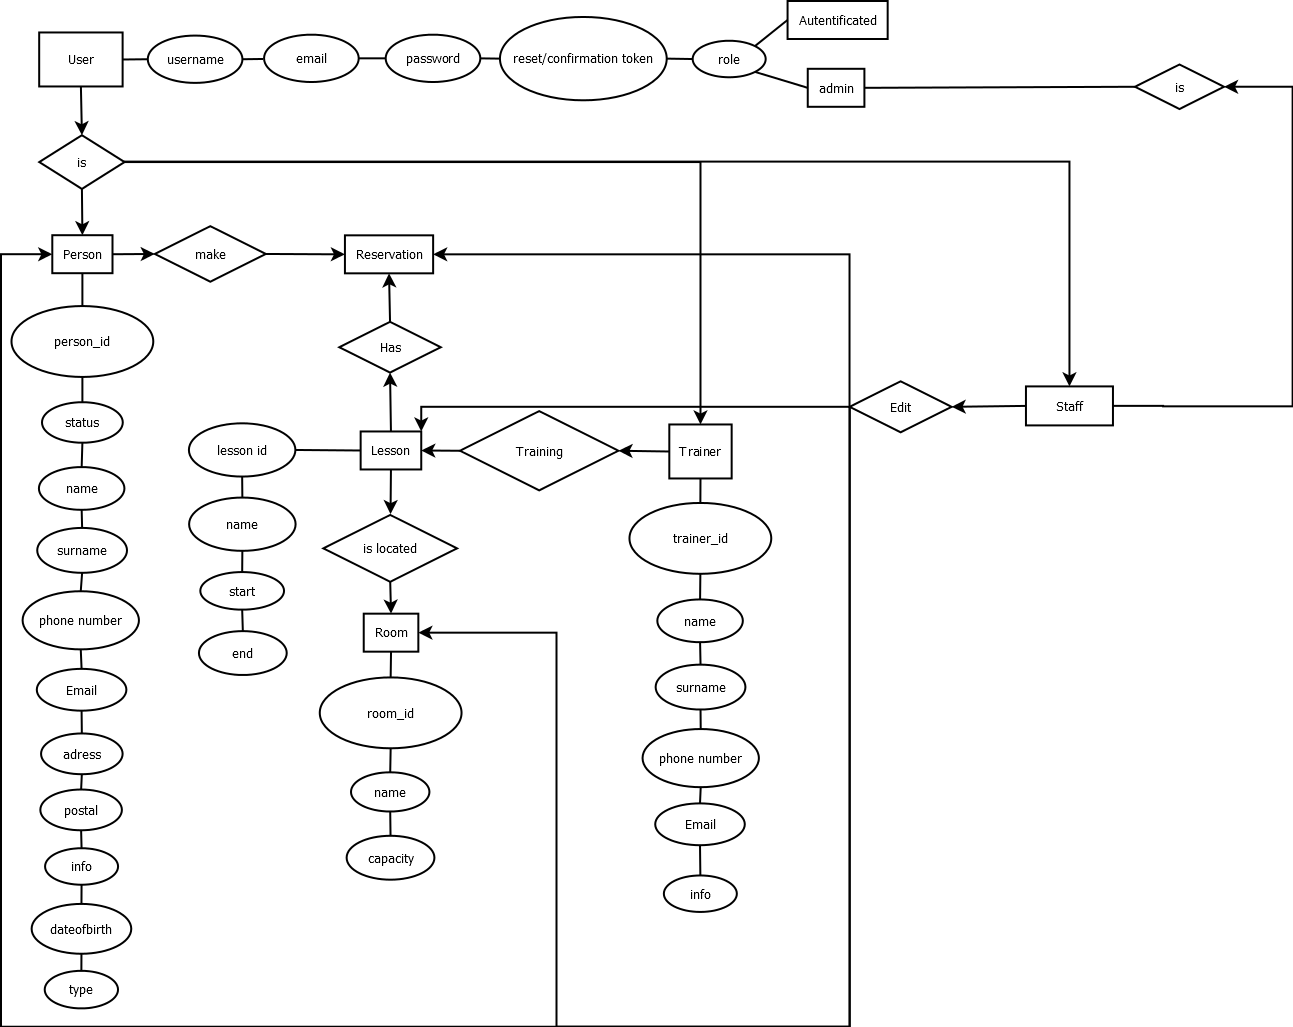
\includegraphics[width=1\linewidth]{image/Diagram.png} 
            \caption{ER diagram}
		\end{figure}

\section{Zkušenosti s tvorbou databází}
\label{sec:zkusenosti}

Problematika databázových aplikací pro mě není problémem. Jelikož tento projekt vychází z~aplikace v Djangu ze třetího ročníku. Dále jsem vycházel ze zkušeností se správou databáze MySQL ve webovém rozhraní phpMyAdmin.

	\chapter{Využité technologie}
	V projektu HealthSync byly využity následující technologie, které zajišťují funkčnost systému, jeho škálovatelnost, bezpečnost a uživatelskou přívětivost.
	
	
	\section{Frontend: Uživatelské rozhraní} 
    
\subsection{Next.js}
Next.js rozšířil možnosti Reactu o server-side rendering (SSR) a generování statických stránek, což vedlo ke zlepšení výkonu aplikace a SEO.
Integrované API routy umožnily jednodušší implementaci komunikace s backendem.
\subsection{CSS Modules}
    CSS Modules byly použity k modularizaci a izolaci stylů, což zamezilo konfliktům mezi různými částmi aplikace.
    
    \section{Backend: Správa dat a autentizace
} 
    
\subsection{Strapi CMS}
Strapi byl nasazen jako hlavní backendový systém díky své jednoduchosti, možnosti rychlé konfigurace a nativní podpoře REST API i GraphQL.
Zajišťuje správu entit, jako jsou uživatelé, lekce, rezervace a místnosti.
Funkce autentizace a oprávnění umožnily snadnou správu přístupu k datům.
\subsection{Node.js}
    Základ backendové logiky a runtime prostředí, které umožňuje škálovatelnost a efektivní zpracování požadavků.

    \section{Databáze} 
    
\subsection{SQLite}
SQLite je lehká a snadno použitelná databáze, která nevyžaduje konfiguraci serveru.
Je vhodná pro projekty s nižšími nároky na paralelní zpracování dat a pro aplikace, kde je kladen důraz na~rychlou a bezproblémovou správu databázových souborů.
\section{Autentizace a autorizace} 
    
\subsection{OAuth 2.0 a JWT}
K zajištění bezpečné autentizace byl použit OAuth 2.0 pro přihlašování pomocí externích služeb (např. Google).
JSON Web Tokens (JWT) slouží k uchování uživatelské relace a k autorizaci přístupů k chráněným zdrojům.

\section{Další technologie} 
    
\subsection{Axios - Fetch API}
Axios a nativní Fetch API byly využity pro komunikaci mezi frontendem a backendem. Tyto knihovny umožnily snadnou práci s REST API.
\subsection{JWT Decode}
Pro dekódování a ověřování JWT tokenů byl použit balíček jwt-decode, což usnadnilo správu uživatelských relací.

    
\clearpage
	
	\chapter{Způsoby řešení a použité postupy}
	
	\section{Backend} 
    Pro backend aplikace jsem použil Node.js společně s frameworkem Strapi, což je headless CMS, který umožňuje snadné vytváření REST API a spravování obsahu. Backend jsem navrhl tak, aby zajišťoval následující funkce:
    
\subsection{Správa dat}
Next.js rozšířil možnosti Reactu o server-side rendering (SSR) a generování statických stránek, což vedlo ke zlepšení výkonu aplikace a SEO.
\begin{itemize}
	\item Vytvoření entit pro lekce, uživatele, místnosti a rezervace. 
	\item Každá entita obsahuje relevantní atributy, například:Lekce: název, čas zahájení, čas ukončení, místnost, trenér.
\end{itemize}
\begin{figure}
    \centering
    \includegraphics[width=0.6\linewidth]{image/Snímek obrazovky 2024-12-27 140428.png}
    \caption{Struktura modelu}
    \label{fig:enter-label}
\end{figure}
\clearpage
\subsection{API pro komunikaci}
    Implementace REST API endpointů umožňujících CRUD operace (vytvoření, čtení, úprava, mazání).Endpoints pro správu lekcí, rezervací a uživatelů, například: /api/lessons pro manipulaci s lekcemi. Pomocí parametrů "?populate=trainer" například vypíše navazující data o trenérovi.

\begin{lstlisting}[style=JavaScript, title={API}, caption={Ukázka API }]
  "data": [
    {
      "id": 5,
      "attributes": {
        "Name": "lesson 2",
        "locale": "cs-CZ",
        "Start": "2024-09-21T18:00:00.000Z",
        "End": "2024-09-21T19:00:00.000Z",
        "trainer": {
          "data": {
            "id": 2,
            "attributes": {
              "name": "trainer",
              "surname": "1",
              "locale": "cs-CZ",
              "email": "trainer2@test.test",
              "info": [
                {
                  "type": "paragraph",
                  "children": [
                    {
                      "type": "text",
                      "text": "geraegyčgyshszSGyhzger"
                    }
                  ]
                }
              ],
              "telephone": "+420 132 789 654"
            }
          }
        },
        "room": {
          "data": {
            "id": 1,
            "attributes": {
              "Name": "Funkční zóna",
              "Capacity": 30,
            }
          }
        }
      }
\end{lstlisting}
    
    \subsection{Autentizace} 
    Použití JWT (JSON Web Token) pro zabezpečení API.
    Uživatelé mohou být registrováni a přihlašováni buď přes Google OAuth nebo pomocí tradičního přihlašovacího mechanismu.
    Ochrana endpointů podle rolí (administrátor má přístup k širším funkcím než klient).
    \begin{lstlisting}[style=JavaScript, title={Kód}, caption={JWT přístup}] 
     // ukladání jwt tokenu pro přístup k api requestům
    try {
      const res = await 
      fetch(`${process.env.NEXT_PUBLIC_API_URL}/api/auth/local`, 
      {
        method: 'POST',
        headers: {
          'Content-Type': 'application/json',
        },
        body: JSON.stringify({
          identifier, // email nebo username
          password,
        }),
      });
      const data = await res.json();

      if (res.ok) {
        // Ukládáni JWT, userId po přihlášení
        localStorage.setItem('jwt', data.jwt);
        localStorage.setItem('userId', data.user.id);
\end{lstlisting}

\clearpage
    \section{Frontend} 
    Frontend byl postaven s použitím Next.js, moderního frameworku pro React.js, který umožňuje server-side rendering a optimalizovaný výkon.
    
\subsection{Přihlašovací a registrační systém}
Uživatelé se mohou registrovat a přihlašovat pomocí Google OAuth nebo e-mailu.
Po přihlášení získávají uživatelé přístup k odpovídajícím funkcím podle svého typu (klient nebo administrátor).
\begin{figure}[h]
    \centering
    \includegraphics[width=1\linewidth]{image/Snímek obrazovky 2024-12-27 141722.png}
    \caption{Příhlašovácí stránka}
    \label{fig:enter-label}
\end{figure}

Přihlášení klasickým způsobem bylo řešeno přímo pomocí Strapi, kterému byly předána pouze data od uživatele při registraci. Při přihlášení přes OAuth nastal problém.
Zde muselo být dořešeno přihlášení přes OAuth, Strapi v základu automaticky nevytvoří uživatele pouze si vezme jeho data z Googlu. Bylo nutné dořešit funkci pro vytvoření uživatele nebo přihlášení uživatele pokud již existuje. Díky tomu bylo dosáhnuto jednoduššího přihlášení/registrace pomocí jednoho tlačítka.

\begin{lstlisting}[style=JavaScript, title={Kód}, caption={Ukázka řešení oauth loginu}, basicstyle=\footnotesize\ttfamily]
	useEffect(() => {
    const params = new URLSearchParams(window.location.search);
    const oauthToken = params.get('id_token'); // Zachycení OAuth tokenu z URL

    if (!oauthToken) {
      setError('Missing ID Token');
      setLoading(false);
      return;
    }

    try {
      // Dekodování JWT tokenu při přístup k uživatelským datům
      const decoded = JSON.parse(atob(oauthToken.split('.')[1])); // Dekodování tokenu
      const userEmail = decoded.email; 

      if (!userEmail) {
        setError('Email not found in the token');
        setLoading(false);
        return;
      }

      // Kontrola pokud uživatel existuje podle emailu
      fetch(`${process.env.NEXT_PUBLIC_API_URL}/api/users?filters[email]=${userEmail}`)
        .then((response) => {
          if (!response.ok) {
            throw new Error(`Failed to fetch user data, Status: ${response.status}`);
          }
          return response.json();
        })
        .then((data) => {
          // pokud existuje
          if (data && data.length > 0) {
            console.log('User found:', data[0]);
            // Step 2: Přihlásí se za nalezeného uživatele v: /api/auth/local
            loginUser(data[0].email, data[0].id);
          } else {
            // Pokud neexistuje, Vytvoří se uživatel.
            createUser(userEmail);
          }
          setLoading(false); 
        })
        .catch((err) => {
          setError(`Error fetching user data: ${err.message}`);
          console.error('Error fetching user data:', err);
          setLoading(false);
        });
    } catch (err) {
      setError('Failed to decode ID Token');
      console.error('Error decoding token', err);
      setLoading(false);
    }
  }, [router]);
\end{lstlisting}
\subsection{Hlavní stránka}
Zde byl vytvořen kalendář lekcí co nejjednodušeji. Kalendář zobrazuje aktuální týden, v nedělních hodinách se automaticky zobrazí týden následující.Každá lekce má detailní stránku kde jsou uvedeny informace o čase, místnosti, trenérovi a seznamu účastníků. Klienti mohou jedním kliknutím rezervovat místo na lekci. Dále mohou na hlavní stránce sledovat následující rezervované lekce a detail profilu (v budoucnu stav peněženky/permanentky).


	        \begin{figure}[h]
	            \centering
	            \includegraphics[width=1\linewidth]{image/Snímek obrazovky 2025-01-07 172741.png}
	            \caption{Hlavní stránka}
	            \label{fig:enter-label}
	        \end{figure}
	    	    
    \begin{lstlisting}[style=Python, caption={Ukázka řešení kalendáře}, basicstyle=\footnotesize\ttfamily]
	const Calendar = ({ lessons, onLessonClick }) => {
  const daysOfWeek = ['Monday', 'Tuesday', 'Wednesday', 'Thursday', 'Friday'
  , 'Saturday', 'Sunday'];
  const timeSlots = Array.from({ length: 15 }, (_, i) => `${i + 8}:00`); 
  //období od 8:00 do 22:00


  return (
    <div className={styles.calendar}>
      <div className={styles.header}>
        <div className={styles.timeCell}></div>
        {daysOfWeek.map(day => (
          <div key={day} className={styles.dayCell}>{day}</div>
        ))}
      </div>
      {timeSlots.map((time) => (
        <div key={time} className={styles.timeRow}>
          <div className={styles.timeCell}>{time}</div>
          {daysOfWeek.map((day) => {
            const lessonForCell = lessons.find((lesson) => {
              const start = new Date(lesson.attributes.Start);
              const end = new Date(lesson.attributes.End);
              const lessonDay = start.toLocaleDateString('en-US', { weekday: 'long' });

              // Kontrola jestli lekce patří do daného dne
              if (lessonDay !== day) return false;

              // Kalkulace počátku a konce lekce
              const startHour = start.getHours() - 1;
              const endHour = end.getHours() - 1;
              console.log(`Lesson: ${lesson.attributes.Name}, Day: ${lessonDay}, 
              Time: ${startHour}-${endHour}`);
              // Kontrola jestli hodina nepřetéká do další buňky
              return (
                (startHour === parseInt(time) && start.getMinutes() > 0) ||
                (endHour === parseInt(time) && end.getMinutes() === 0) ||
                (startHour < parseInt(time) && endHour > parseInt(time))
              );
            });

            return (
              <div key={day} className={`${styles.lessonCell} 
              ${lessonForCell ? styles.hasLesson : ''}`}>
                {lessonForCell && (
                  <div
                    className={styles.lessonContent}
                    onClick={() => onLessonClick(lessonForCell)} // Click handler
                  >
                    {lessonForCell.attributes.Name}
                  </div>
                )}
              </div>
            );
          })}
        </div>
      ))}
    </div>
  );
};
\end{lstlisting}
\clearpage
    \subsection{Administrace}
    Administrace byla klíčovým prvkem celého systému i celého mého projektu.
    Po přihlášení má administrátor možnost vytvářet, mazat a upravovat lekce, místnosti a uživatelské profily.
    Jedná se o přehlednou administraci, která zobrazuje všechny klíčové údaje na jednom místě s možností hledání či filtrů pomocí měsíců nebo týdnů. Na druhém obrázku je možnost vidět konkrétní uživatelé přihlášené na lekci, manuálně je vyhledat, přidat nebo rezervaci zrušit.
    
    \begin{figure}[h]
    \centering
    \begin{minipage}{0.45\textwidth}
        \centering
        \includegraphics[width=1\linewidth]{image/Snímek obrazovky 2025-01-07 172938.png}
        \caption{Seznam lekcí}
        \label{fig:image1}
    \end{minipage}
    \hfill
    \begin{minipage}{0.45\textwidth}
        \centering
        \includegraphics[width=1\linewidth]{image/Snímek obrazovky 2025-01-07 173141.png}
        \caption{Seznam rezervací na lekci}
        \label{fig:image2}
    \end{minipage}
    \end{figure}
    \clearpage
        Úprava dat je ošetřena tak, aby nebylo možno zadávat neplatná data u emailu, tel. čísla ve~špatném tvaru, psč. Bylo ošetřeno taktéž překročení maximální kapacity u rezervace lekce.
        \begin{figure}[h!]
            \centering
            \includegraphics[width=1\linewidth]{image/Snímek obrazovky 2025-01-07 174728.png}
            \caption{Maximální počet rezervací}
            \label{fig:enter-label}
        \end{figure}
\begin{figure}[h!]
    \centering
    \includegraphics[width=1\linewidth]{image/Snímek obrazovky 2025-01-07 175059.png}
    \caption{Ošetření}
    \label{fig:enter-label}
\end{figure}



\chapter{Výsledky a zhodnocení}
\subsection{Splněné cíle}
Na začátku projektu byly definovány jasné cíle, jejichž dosažení mělo zajistit funkční a uživatelsky přívětivý rezervační systém.
\begin{itemize}
	\item Vytvoření webové aplikace s uživatelským rozhraním pro klienty i administrátory.
	\item Implementace přihlášení uživatelů pomocí OAuth 2.0 (Google) a klasické registrace.
    \item Zobrazení dostupných lekcí v přehledném kalendáři s možností detailního náhledu.
    \item Administrátorský přístup umožňující správu uživatelů, lekcí a místností.
    \item Použití responzivního designu pro snadné ovládání na mobilních zařízeních.
    \item Vytvořit pevný základ pro možné budoucí rozšíření.
\end{itemize}


\subsection{Budoucí rozvoj}
Ačkoli je aplikace v současné podobě plně funkční, existují další možnosti rozšíření, které by mohly zlepšit uživatelskou zkušenost i technickou stránku systému. Mezi nejdůležitější plánované kroky pro budoucí rozvoj patří:
\begin{itemize}
\item Implementace notifikací: Přidání e-mailových a push notifikací pro upozornění na rezervace a změny v rozvrhu.
\item Platby online: Integrace platební brány pro snadné platby přímo v aplikaci.
\item Statistiky a reporty: Vytvoření analytických nástrojů pro sledování obsazenosti lekcí a preferencí uživatelů.
\item Víceúrovňová správa uživatelů: Zavedení dalších rolí, například trenérů, s přístupem pouze k jejich vlastním lekcím.
\item Eshop: Nákup permanentek dobíjení kreditu atd.
\item Změna použité technologie na backend (Strapi je naprosto jednoduchý systém pro učení, ale bohužel k nasazení do reálného provozu je příliš pomalý a chybí zde pokročilejší funkce pro vývoj backendu.)
\item Implementace do webových stránek: Posledním krokem by byl redesign celých webových stránek a implementace rezervačního systému
\item Navázání systému: navázání na odbavovací systém, později i vytvoření celého interního odbavovacího/pokladního systému navázaného na web a rezervační systém.
\end{itemize}
\subsection{Zhodnocení}
Projekt přinesl mnoho výzev, ale také příležitostí k rozšíření znalostí a dovedností.
Hlavním přínosem projektu je vytvoření plně funkčního systému, který zjednodušuje proces rezervací a přináší větší komfort uživatelům i administrátorům.

Na druhou stranu projekt odhalil několik oblastí pro zlepšení, například potřebu hlubší optimalizace backendu a rozšíření API o pokročilejší funkcionality. Tyto nedostatky jsou však plánovány k odstranění v budoucích verzích aplikace.

Projekt lze hodnotit jako úspěšný, protože splnil definované cíle a přinesl užitečný nástroj. Navíc položil pevné základy pro budoucí rozvoj a další vylepšení.

        
				\chapter*{Závěr}
                Vytvoření tohoto rezervačního systému bylo náročným, ale zároveň velmi přínosným procesem. Cílem projektu bylo navrhnout a implementovat moderní webovou aplikaci, která zjednoduší proces rezervací a přinese větší pohodlí jak uživatelům, tak administrátorům. Projekt nejenže splnil všechny stanovené cíle, ale poskytl také příležitost pro rozšíření odborných znalostí a dovedností v oblasti vývoje webových aplikací.

Aplikace v aktuální podobě nabízí intuitivní uživatelské rozhraní, efektivní správu rezervací a přístupné administrátorské funkce. Díky integraci OAuth 2.0 pro přihlášení a využití moderních technologií, jako je React.js a Strapi.js, bylo dosaženo vysoké úrovně uživatelského komfortu a technické spolehlivosti.

Z praktického hlediska přináší aplikace mnoho výhod. Umožňuje rychle a snadno rezervovat lekce, spravovat uživatelské účty a plánovat události. Z administrátorského pohledu systém snižuje pracovní zátěž a zajišťuje přehlednost.

Během realizace projektu se ukázalo, že některé oblasti vyžadují další rozvoj. Patří mezi ně například rozšíření o pokročilé analytické funkce, integrace notifikací nebo podpora více jazyků. Tyto kroky však představují další fáze, na které je aplikace technicky připravena.
	
Zdrojový kód projektu:(\url{https://github.com/Endru88/zaverecny-projekt})
	
	%% literatura
    \renewcommand{\bibname}{Seznam použitých zdrojů}
	\begin{thebibliography}{99}
		\bibitem SSTRAPI \textit{Strapi Documentation} [Online]. 2024. Dostupné z: \url{https://docs.strapi.io/dev-docs/intro}
        \bibitem SNEXTJS \textit{NextJs Documentation} [Online]. 2024. Dostupné z: \url{https://nextjs.org/docs}
        \bibitem SNODEJS \textit{NodeJs Documentation} [Online]. 2024. Dostupné z: \url{https://nodejs.org/docs/latest/api/}
        \bibitem YYOUTUBE TUTORIALY \textit{Strapi tutorials} [Online]. 2024. Dostupné z: \url{https://www.youtube.com/@Strapi}
        
        \bibitem EEXAMPLE \textit{Strapi+NextJs Example} [Online]. 2024. Dostupné z: \url{https://github.com/buraste/strapi-nextjs-docker-boilerplate}
		
	\end{thebibliography}
	
	
	
	\appendix %% začínají přílohy
	
	\titleformat{\chapter}[block]{\scshape\bfseries\LARGE}{Příloha \thechapter}{10pt}{\vspace{0pt}}[\vspace{-22pt}] %% nastavení nadpisu u příloh
	
	
	




	
	

	
	
\end{document}